\chapter{Tecnología en el Proceso Electoral}
\label{SistemaElectoral}
%\cambiar{No se describen todos los sistemas de votos existentes, y si se hace, están en forma muy resumida. No analiza ventajas y desventajas de cada uno (2.1.1). No se analizan los votos en papel sin uso de tecnología. - RESPONDIDO EN DOC}

%\cambiar{Describe mecanismos de voto electrónico, pero no con sus características, sino con ejemplos de implementación. Deberían ser dos cosas diferentes. - HECHO: se sacan los ejemplos}
%\cambiar{Faltan referencias que respalden los conceptos plasmados y las opiniones. En general se dan muchas opiniones, en su mayoría negativas, de los sistemas electorales nombrados sin fundamentos. Es decir, son opiniones del autor? se han analizado? - RESPONDIDO EN DOC}
%\cambiar{A veces dice Figura, otras Gráfico, otras Imágen. Unificar Figura. - HECHO}
%\cambiar{En general: El capítulo advierte de una revisión conceptual de las características de un sistema electoral tradicional (según Capítulo 1). Sin embargo, luego se mezcla con la aplicación de tecnologías al sistema. No analiza y compara los sistemas de votos. Da opiniones sin fundamento.}

Involucrar tecnología en el proceso electoral es complejo, no sólo por sus desafíos técnicos, sino también por su importancia para el Estado y para la sociedad en general. Un sistema de voto electrónico involucra considerar aspectos de software, hardware, procesos operativos, y personas. Por lo tanto, cualquier desarrollo debe tener el aspecto de calidad como el objetivo más importante en el proceso.\newline
%\agregar{cita a texto del Ministerio - ESTO SALIÓ DEL DOCUMENTO DE CONICET Un sistema de votación debe considerar los siguientes objetivos \cite{conicet}: - HECHO}
Un sistema de votación debe considerar los siguientes objetivos \cite{conicet}:
\begin{itemize}
    \item Garantizar la completitud en la oferta electoral
    \item Simplificar el uso de boletas (por ej. con boleta única)
    \item Brindar mayor accesibilidad a los ciudadanos a la hora de votar (por ej. para personas con alguna discapacidad)
    \item Lograr precisión y rapidez en el proceso de conteo de votos
\end{itemize}
Además un sistema de votación que incorpore algún grado de automatización debe construir la confianza de los ciudadanos, partidos políticos y gobierno, en el sistema y en el proceso de votación \cite{conicet}.

Una de las ventajas más deseadas en automatizar el proceso es la rapidez en el conteo. Si todo sale bien los resultados pueden ser inmediatos pero el problema es el impacto que pueden generar las distintas ``cosas'' que pueden salir mal. La rapidez sin confianza ni seguridad no es útil para cualquier proceso electoral y por esto es que la eficacia debe importar por sobre la eficiencia o rapidez.

\section{Sistema electoral}

Un sistema electoral consiste de reglas y procedimientos técnicos que producen determinadas consecuencias, es decir, los sistemas electorales no son neutros. 
La complejidad es afectada por la cantidad de representantes que se eligen por distrito electoral y la forma de votación. El voto se realiza a través de las boletas electorales, instrumento importante por el cual el ciudadano expresa su voluntad, además de ser la prueba real del voto y el medio para realizar el recuento de votos o escrutinio.
Actualmente las condiciones jurídicas del sufragio están constituidas por su universalidad, igualdad, obligatoriedad y secreto. Sin embargo, en Argentina para llegar a ese punto, los condicionamientos y las formas de votar fueron modificándose a través de la historia.

En 1873 el voto oral se convirtió en voto escrito, luego ha sufrido modificaciones hasta el año 1995, cuando la reforma de la Constitución Nacional define el régimen electoral actual quedando de la siguiente manera \cite{historia}:
\begin{itemize}
    \item Sistema de Representación Proporcional
    \item Método de Conversión de votos en escaños: Sistema D'Hondt \cite{flis2020pot}
    \item Umbral 3\% del padrón electoral de distrito
    \item La elección de todos los representantes argentinos se eligen en forma directa por el pueblo de la Nación Argentina.
\end{itemize}
\newline


\section{Propiedades de Calidad}
\label{propiedadesCalidad}
%\cambiar{Sección 2.2. No están claras las propiedades nombradas. No las explica, sino que las compara con sistemas que no fueron descriptos. - HECHO: Se cambio la seccion de las propiedades, se quitaron las experiencias y solo se dejó la explicacion de cada uno}
Para lograr un sistema electoral exitoso y confiable a la vista de las partes involucradas es necesario que cumpla ciertas propiedades de calidad, sin tener en cuenta si este proceso incluye tecnología o no. A continuación se enumeran estas propiedades que todo sistema electoral debe satisfacer.
%\agregar{Párrafo marco sobre Atributos de Calidad - HECHO?}
%\cambiar{A partir de las partes involucradas en el proceso surgen distintas propiedades a satisfacer un sistema electoral con o sin tecnología, que se describen a continuación. - HECHO}
\begin{itemize}
    \item Secreto del voto: El sistema debe garantizar que sólo el votante tiene conocimiento del contenido de su voto. La sola sospecha de que alguien pueda conocer el contenido de su voto impide la libre emisión del sufragio.
    \item Integridad: El sistema debe garantizar que la cadena de confianza no puede romperse. Esta propiedad se encuentra ligada a la seguridad del sistema para proteger datos e información de accesos no autorizados, pero proveyendo al mismo tiempo acceso a personal autorizado para operar.
    \item Capacidad de auditoría y control del proceso electoral: Se debe poder monitorear el sistema tanto en su diseño (estructura), en funcionamiento (ejecución) y cuando ya dejó de utilizarse (análisis post-hoc). Un sistema de votación debe poderse auditar en todos sus niveles sin afectar los atributos de secreto e integridad.
    \item Igualdad de condiciones para todos los partidos políticos: El sistema debe garantizar que la oferta electoral se encuentre en igual de condiciones hacia los votantes, sin preferencia o prioridad, sobre la mesa de votación. Particularmente esta propiedad puede resultar difícil de cumplir en una pantalla o monitor debido a las limitaciones físicas.
    \item Universalidad: El sistema debe estar preparado para facilitar el sufragio de toda persona habilitada, esto incluye personas con requerimientos de accesibilidad, por ejemplo no videntes. Debemos tener en cuenta que toda persona posee los mismos derechos sobre el voto.
    \item Usabilidad: El sistema debe ser fácil e intuitivo para cualquier persona involucrada en el proceso de la elección. Esta propiedad también ayuda al objetivo de rapidez ya que un sistema difícil de entender generará largas colas de espera para votar porque a varias personas les lleva tiempo entender y generar su sufragio. De igual manera mejoraría los tiempos del escrutinio realizado por cada autoridad de mesa.
    \item Cumplir con las normativas vigentes del proceso electoral: Un proceso electoral regularmente no modifica sus políticas o reglas que lo conforman. De todos modos, un sistema debe ser capaz de adaptarse a cualquier cambio adoptado por las autoridades de un país, provincia o distrito.
\end{itemize}
Un sistema electoral que incluya tecnología debe poder cumplir todas las propiedades de calidad, algo dificil de lograr. Por ejemplo se ha demostrado que satisfacer los atributos de integridad, auditabilidad y secreto simultáneamente es complejo y es una tarea imposible de cumplir \cite{vora}. Cualquier sistema de voto electrónico que intente solucionar los problemas inherentes a garantizar integridad y secreto, estará en una situación difícil para lograr una verificación formal y en auditabilidad \cite{conicet}.
Además, los aspectos de Seguridad Informática cobran gran importancia si es un sistema de misión crítica, un error en el sistema que pueda ser explotado por un atacante podría atentar contra alguna de las propiedades del voto o el resultado de la votación en general.


\begin{comment}
\subsection{Secreto del voto}

\subsection{Integridad}
Requiere garantizar que la cadena de confianza no puede romperse. Esta propiedad también se encuentra ligada a la seguridad del sistema para proteger datos e información de accesos no autorizados, pero proveyendo al mismo tiempo acceso a personal autorizado para operar. En particular, se consideran importantes las propiedades de confidencialidad, integridad, disponibilidad y autenticidad. Los aspectos de Seguridad Informática cobran gran importancia en un sistema de misión crítica, un error en el sistema que pueda ser explotado por un atacante podría atentar contra alguno de los principios básicos del voto o el resultado de la votación en general. Frente a esto, tenemos el ejemplo de las elecciones en Holanda que a partir de 1997 se votaba con el sistema fabricado por la empresa Nedap. Luego de 9 años un grupo de activistas demostró en un programa de televisión las vulnerabilidades del sistema. Esto generó que el gobierno decidiera volver al sistema tradicional en papel \cite{eleccionesHolanda}. 
Otro ejemplo serian las elecciones presidenciales de EEUU, como en el 2004 y las últimas elecciones en el 2020, en las que las diferencias entre las encuestas en boca de urna y los resultados finales sugieren fuertemente que las urnas dieron resultados dudosos.\newline
Esta propiedad incluye capturar la intención del voto de manera fehaciente (y sin introducir sesgos), registrar la intención de voto exactamente como fue capturada, garantizando que se respeta la voluntad de cada votante, es decir que el sistema no permita cambiar el voto una vez que el votante lo emitió, y contabilizar el voto exactamente como fue registrado. Si el sistema, por error o ataque, altera la suma de los votos individuales lo hará de una forma que será evidente para los ciudadanos.

\subsection{Capacidad de auditoría y control del proceso electoral (sin afectar los atributos de secreto e integridad anteriores)}
Capacidad de monitorear el sistema tanto en su diseño (estructura), como cuando se encuentra en funcionamiento (ejecución) y cuando ya dejó de utilizarse (análisis post-hoc). Un sistema de votación debe poderse auditar en todos los niveles de hardware y software. El principio rector es que 
``las elecciones deben dar una evidencia consistente de un resultado preciso, aún cuando el rival sea quien escribe el software, administra la elección o gobierna el país''.\newline
En el sistema de votación tradicional, la responsabilidad de auditoría está distribuida en todos porque todos pueden ver y entender el sistema. Lejos de aportar transparencia, la urna electrónica obstaculiza la capacidad de la mayoría de los ciudadanos de fiscalizar la elección, ya que queda necesariamente en manos de una élite tecnológica a la que el resto de la población no le queda otra que creerle.

Este fue el caso del estado de Georgia en EEUU que a partir del 2002 y hasta el 2019 las elecciones fueron cien por ciento electrónicas y con el mismo tipo de máquinas. Esto quiere decir que gran parte de los votos no tiene recuento posible ya que no existe comprobante físico para contabilizar \cite{eleccionesGeorgia}.\newline
La incorporación de urnas electrónicas tiene efectos contrarios a este objetivo ya que las personas con poca afinidad con los sistemas computacionales (adultos mayores, personas de escasos recursos, con dificultad visual, entre otras) se verán enfrentados a un sistema mucho más complejo para votar. Por otra parte, las personas que auditan las elecciones (maestras de escuela, empleados públicos, fiscales de partidos políticos) se verán incapaces de auditar eficazmente este tipo de sistema. Sólo un grupo reducido de personas relacionadas al área de sistemas computacionales comprenderán el funcionamiento de estos sistemas, pero dificilmente se atreverán a firmar a conciencia una certificación de seguridad de las urnas pues, no existe método formal de validación que los avale. Si bien no existen sistemas perfectos, la diferencia de impacto es sustancial. Un error mínimo en un sistema de votación electrónica puede alterar el resultado de una elección en un gran número de mesas simultáneamente.

\subsection{Igualdad de condiciones para todos los partidos políticos}
Todo sistema electrónico tiene un límite técnico donde manipular o visualizar la oferta electoral. Como ejemplo tenemos las elecciones del 2019 que se llevaron a cabo en Neuquén y Plottier para los comicios municipales (como muestra la Figura \ref{graf:buenqn}). En el caso de Plottier se debieron distribuir 29 listas en una pantalla con capacidad de 18 casilleros. Lograr distribuir la totalidad de las listas implicó que no exista ventaja entre candidatos por las maniobras de mercantilizar la herramienta de las colectoras \cite{limiteColectoras}.

\begin{figure}[h!]
    \begin{center}
        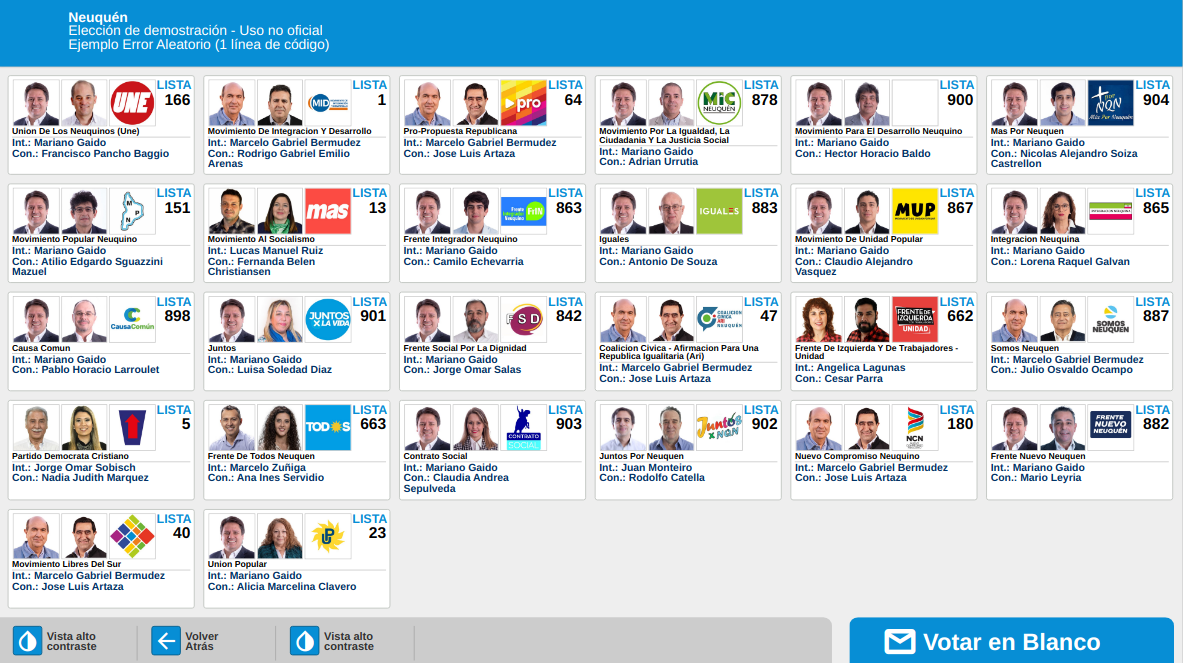
\includegraphics[width=\textwidth]{img/buenqn2019.png}
    \end{center}
  \caption{Pantalla del sistema BUE utilizado en las Elecciones Municipales de Neuquen 2019}
  \label{graf:buenqn}
\end{figure}

\subsection{Universalidad}
El sistema debe estar preparado para facilitar el sufragio de toda persona habilitada, esto incluye personas con requerimientos de accesibilidad, por ej. no videntes. Debemos tener en cuenta que toda persona posee los mismos derechos sobre el voto. Por lo tanto, si se requiere el acompañamiento debido a la complejidad o inaccesibilidad del sistema no se está alcanzando ninguna ventaja por sobre el sistema electoral tradicional.\newline
Como ejemplo, las máquinas usadas en elecciones electrónicas en general se basan en fotos y colores como medio de accesibilidad para las personas que no puedan leer o con baja visión. Por otro lado, en varios paises es común la instalación de un kit accesible como un teclado especial y auriculares para personas invidentes.

\subsection{Usabilidad}
El sistema debe ser fácil e intuitivo para cualquier persona involucrada en el proceso de la elección. Un sistema electrónico debe ser fácil de aprender tanto para un votante como para las autoridades encargadas de dar soporte. Esta propiedad también ayuda al objetivo de rapidez ya que un sistema difícil de entender generará largas colas de espera para votar debido a que varias personas les lleva más tiempo entender y generar su sufragio. De igual manera la facilidad de uso mejoraría los tiempos del escrutinio realizado por cada autoridad de mesa.

\subsection{Cumplir con las normativas vigentes del proceso electoral}
Un sistema electoral regularmente no modifica sus políticas o reglas que lo conforman. De todos modos, un sistema de votación electrónica debe ser capaz de adaptarse a cualquier cambio adoptado por las autoridades de un país, provincia o distrito.

\subsection{Integridad vs. Auditabilidad vs. Secreto}
En todo sistema electoral (sea en formato de papel o electrónico) se ha demostrado que satisfacer los atributos de integridad, auditabilidad y secreto simultáneamente es complejo y es una tarea imposible de cumplir. Cualquier sistema de voto electrónico que intente solucionar los problemas inherentes a garantizar integridad y secreto, estará en una situación difícil para lograr una verificación formal y en auditabilidad. \cite{conicet}

\end{comment}


\subsection{Clasificación de Sistemas de Voto Electrónico}
\label{ClasificacionVotoElectronico}

En el sistema electoral existen partes del proceso vulnerables a la incorporación de recursos informáticos con el objetivo de agilizar su ejecución. Como concepto general, se considera ``voto electrónico'' a todo sistema electoral que incorpore tecnología en las fases de emisión y recuento de votos de la mesa de votación, de otro modo, se le denomina simplemente sistema de votación electrónica.

Experiencias de voto electrónico en distintos puntos del país y en otros países implementaron variadas técnicas con distintos impactos de aceptación o rechazo logrando unos cuantos intentos para finalmente volver al sistema electoral tradicional. Se identifican 3 grandes mecanismos.
%\propuesta{Separado por subsubseccion}
\subsubsection{Reconocimiento óptico de boletas}
El recuento es automático mediante el escaneo de marcas especiales aplicadas por los ciudadanos sobre las boletas. Estas marcas pueden ser perforaciones (tarjetas perforadas) o boletas impresas en papel que el elector debe rellenar para luego ser contabilizado mediante reconocimiento óptico de caracteres. %Los primeros sistemas datan del siglo XIX en Nueva York mediante tarjetas perforadas. Por otro lado, en Venezuela implementaron la segunda opción con boletas en papel en sus elecciones desde 1994 hasta 2003 \cite{eleccionesVenezuela}.
\begin{itemize}
    \item Ventajas: Conservar el principio de mantener la voluntad del elector en un trozo de papel anónimo fácilmente auditable independiente de los dispositivos y software usados.
    \item Desventajas: Suponen un doble trabajo para el votante (elegir y además controlar que su elección sea correctamente impresa). Pone en riesgo el anonimato del voto al poder agregar “suciedad” que en realidad codifique información permitiendo reconstruir la emisión de los votos y la relación de cada votante con su voto. Otro posible problema, el escáner puede fallar en la lectura de cierto tipo de tinta utilizada por el votante \cite{RecuentoAutomaticoFallas}. \newline
\end{itemize}
Si bien cualquier sistema basado en papel podría ser adulterado, esto debe ser hecho individualmente con cada boleta, y el impacto de una persona corrupta se limita a las boletas bajo su custodia. En el sistema electrónico, en cambio, una única persona corrupta tiene el potencial de influenciar sobre un gran número de máquinas, comprometiendo la integridad de votos en masa, incluyendo los de las mesas cuyos fiscales actúen de buena fe \cite{libroVoto}.

\subsubsection{Sistema de Registro Electrónico Directo (DRE)}
Los sistemas DRE, también conocidas como urnas electrónicas, ejecutan simultáneamente el registro y la tabulación del voto mediante un dispositivo informático operado por el votante, a través de un teclado, botonera o teclado táctil. Esta acción registra el voto directamente en la memoria del dispositivo. Por lo tanto, se utiliza una sola máquina por mesa de votación encargada de registrar el voto y contabilizarlo. 
\begin{itemize}
    \item Ventajas: Elimina por completo el uso de papel, no hay boletas que custodiar.
    \item Desventajas: Además de poner en riesgo el secreto del voto, dificulta la fiscalización de la integridad del voto al no existir una separación entre el votante y el escrutinio, por lo tanto, poder reconocer una falla o un error es muy difícil de descubrir a tiempo \cite{DRE-Fallas}. 
\end{itemize}
Este mecanismo genera un punto de tensión entre los ciudadanos que necesitan que el resultado refleje sus elecciones y los encargados de conducirlos, que desean terminar la tarea con mayor rapidez y menor esfuerzo delegando toda la responsabilidad a las urnas. La urna electrónica obstaculiza la capacidad de la mayoría de los ciudadanos de fiscalizar la elección, ya que queda necesariamente en manos de una élite tecnológica a la que el resto de la población no le queda otra que creerle \cite{libroVoto}.

\subsubsection{Sistema de votación a distancia}
El votante registra su voto a través de Internet eliminando la presencia del elector en un establecimiento público. 

\begin{itemize}
    \item Ventajas: Elimina por completo el uso de papel.
    \item Desventajas: No existe autoridad encargada de controlar la expresión del elector, identificar que un votante solo vote una única vez, impedir que vote a nombre de otra persona, o no esté habilitado para votar. 
\end{itemize}
Estos sistemas obligan a que la máquina que recibe el voto tenga conocimiento de quien lo está emitiendo, generando un punto de ataque para quien quiera violar el secreto del voto \cite{valdes2010voto}.

\section{Modelo de Referencia}

Mediante el análisis realizado por el Conicet \cite{conicet}, en todo sistema de votación se pueden determinar cinco fases secuenciales del proceso susceptibles de ser automatizada (Figura \ref{graf:modeloDeReferencia}) . Las fases están derivadas del Código Electoral Nacional (Decreto nº2135, 1983) \cite{decreto}

\begin{figure}[h!]
    \begin{center}
        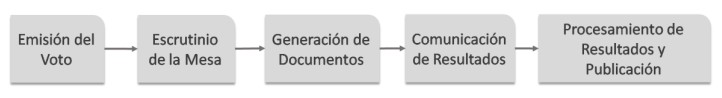
\includegraphics[width=\textwidth]{img/modeloReferencia.png}
    \end{center}
  \caption{Modelo de Referencia}
  \label{graf:modeloDeReferencia}
\end{figure}

%\agregar{Agregar imágen del modelo de referencia - HECHO}
%\cambiar{Está muy textual del artículo del CONICET (Modelo de Referencia, Comunicación de los resultados...., Conteo, Costo en tecnología),  Hay que parafrasear. Sacar la experiencia de los miembros de la Comisión - HECHO}
A continuación se analizan los riesgos y factibilidad técnica de las fases del modelo de referencia teniendo en cuenta distintas fuentes de información, como son los atributos de calidad.

%\cambiar{el orden de las subsecciones por el orden cronológico - HECHO:  el orden es por riesgo}
\subsection{Emisión del Voto} 

En la fase de Emisión del Voto, como su nombre indica, el votante expresa y registra su intención de voto. Esta fase incluye los atributos de calidad de universalidad y secreto del voto, igualdad de condiciones para la oferta electoral, integridad y usabilidad descritas al comienzo del presente capítulo. Como se definió en la sección \ref{ClasificacionVotoElectronico}, cuando existe un dispositivo electrónico como intermediario entre el votante y su intención de voto se denomina al sistema como ``voto electrónico''. La limitación técnica de este sistema es lograr mantener la confidencialidad del emisor del voto sin afectar la posibilidad de verificar si un voto fue emitido válidamente por un ciudadano habilitado o el voto registrado es consecuencia de un mal funcionamiento del sistema. Uno de los motivos por los cuales se intenta incluir tecnología en esta fase es agilizar la velocidad de carga, sin embargo, integrar tecnología en esta fase involucra un alto riesgo, un sistema distribuido de misión crítica es sumamente vulnerable a que una falla en un conjunto o todos los componentes que lo integran produzca un impacto general a todo el proceso electoral. Además una falla en esta fase (detectable o no) se puede propagar fácilmente a las siguientes fases del modelo de referencia. 

Los riesgos que implica una máquina de emisión del voto a nivel de hardware son:
\begin{itemize}
    \item La máquina no está operativa.
    \item Manipulación para modificar la intención del voto.
    \item Manipulación en el guardado y/o transmisión de información adicional que permita posteriormente asociar al elector con su voto.
    \item Manipulación para alterar la representación de la oferta electoral.
    \item Se reemplazó por otro hardware no autorizado indistinguible por los usuarios.
\end{itemize}
%\cambiar{pk: y otros items descritos en articulo de Conicet ¿cuales? agregarlos o sacar la oración - HECHO}
Al ser una fase muy crítica esta máquina de emisión debe tener un diseño y construcción robusta para resistir manipulaciones maliciosas y vandalismo. Por lo tanto, existen ciertos requerimientos mínimos a nivel técnico del hardware como por ejemplo no debe tener almacenamiento estático (disco rígido, SSD, etc.), los componentes no deben ser accesibles salvo únicamente a través de la interfaz del usuario, para evitar comunicaciones PLC (Power Line Communications) \cite{plc} se debe filtrar toda conexión a la red eléctrica, es preferible el uso de baterías, no poseer memoria flash ni otro tipo de memoria no-volátil accesible en ejecución \cite{conicet}.

\subsection{Escrutinio de la Mesa} 
Esta fase consiste en totalizar los datos por categoría y partido político. Este proceso necesita que cada autoridad de mesa realice el recuento independiente y auditado para finalizar en una o más actas con la misma información de la totalización. Incorporar tecnología sólo en esta fase deberá ser únicamente para asistir en el conteo y que su resultado sea una primera aproximación. Como se definió en la sección \ref{ClasificacionVotoElectronico}, incorporar tecnología en esta fase se denomina al sistema como ``voto electrónico''. El resultado final del conteo deberá ser plasmado en las actas con el dato obtenido por conteo manual y así cumplir el principio de independencia del software. 
Este conteo computarizado ayuda a las autoridades de mesa a aumentar su confianza en el resultado del conteo si coincide la cuenta manual con la cuenta electrónica, de todos modos se debe obligar a hacer el conteo manual y no colocar toda la confianza en la tecnología.
Con respecto al hardware, esta fase corre el riesgo de que la máquina no se encuentre operativa o que sea manipulada para cambiar su comportamiento o que sea dañada completamente. Teniendo en cuenta estos problemas se debe tomar algunos recaudos a nivel hardware:
%\cambiar{pk: Agregar otros items....o bien resumirlos en una oración - HECHO}
    \begin{itemize}
        \item No poseer comunicación cableada o inalámbrica accesibles externamente.
        \item Preferiblemente usar baterías para evitar posibles comunicaciones PLC a través de la conexión a la red eléctrica.
        \item Mecanismos de seguridad evitando toda descarga de datos no autorizada.
        \item Separación física entre memoria de datos y memoria de instrucciones de proceso.
        \item Evitar cualquier intercambio de componentes al utilizar algún material con fuerte adherencia.
        \item Inmunidad a un ataque electromagnético moderado.
    \end{itemize}
    
\subsection{Generación de Documentos} 
La fase de Generación de Documentos inicia al momento que se dispone con el resultado del escrutinio de la mesa y finaliza con las actas, certificados y telegramas de escrutinio, todos estos firmados por las autoridades de mesa. En esta etapa es viable incorporar tecnología ya que puede mejorar el desempeño de la generación de estos documentos y en la verificación por parte de los partidos políticos. 
Sin embargo, puede afectar a la integridad de los documentos, los formatos impresos pueden no coincidir con los datos digitales y su detección puede ocurrir luego que se publicaron los resultados provisorios de la mesa. Este riesgo no es fácil de evitar aunque no afectaría al resultado del escrutinio definitivo. 
Con respecto al hardware, la máquina encargada de generar los documentos puede presentar problemas como: 
\begin{itemize}
    \item No estar operativa.
    \item No poder generar o imprimir los documentos.
    \item No poder enviar los documentos electrónicos.
    \item Alterar los documentos electrónicos en tránsito.
\end{itemize}
Como se puede ver, los riesgos están relacionados al mecanismo de transmisión, por lo tanto no requiere un control de seguridad tan estricto como las fases anteriores del modelo de referencia. Relacionado al aspecto técnico del hardware se debería considerar que la máquina no posea puertos de comunicación cableado o inalámbricos accesibles externamente, además debería existir una separación física entre la memoria de datos y la memoria de instrucciones de proceso. 

\subsection{Comunicación de Resultados}

La fase de Comunicación de Resultados implica la transmisión de datos desde el lugar de votación hacia el centro de cómputos. En un sistema de votación cada autoridad de mesa cuenta con un telegrama de escrutinio correspondiente a su mesa firmado. Reducir demoras en la transmisión de estos telegramas es viable debido a que su digitalización y transmisión son realizados desde el mismo lugar de votación. 

Esta transmisión incrementa las propiedades de confiabilidad y verificabilidad del sistema si se transmite tanto la imagen del telegrama como la información contenida. De tal manera, cualquier ciudadano podrá contrastar la información digital con la imagen del telegrama y poder así determinar si existen inconsistencias entre lo impreso y lo digital.

Contar con un soporte digital del telegrama evita la carga centralizada y manual de los datos en el centro de procesamiento. Otra ventaja de contar con la imagen del telegrama y la información digital es que el resultado de la mesa se podría publicar directamente sin necesidad de ninguna intervención humana. Por supuesto, esta situación ideal requiere una evaluación más cuidadosa, ya que está en juego la integridad de los datos, por lo tanto, si esta integridad fue manipulada y los datos digitales no coinciden con lo impreso o cualquier otra situación anómala (por ejemplo la falta de firmas en el telegrama, o números impresos difíciles de distinguir) pondrá en duda la confiabilidad del sistema. Como alternativa a esta situación es útil incorporar un proceso de validación de los datos.


\subsection{Procesamiento de Resultados y Publicación}

En la fase de Procesamiento de Resultados, el centro de procesamientos recibe los datos obtenidos desde cada punto de votación. Estos datos ingresan, se consolida la información y se anuncian públicamente los resultados provisorios y finales. Involucran las interacciones para validar los datos, contrastar con el acta en papel y corregir cualquier desvío. Esta fase incluye los atributos de calidad de integridad, cumplir con las normativas vigentes y auditabilidad descritas al comienzo del presente capítulo. 

Incorporar tecnología sólo en esta etapa, manteniendo en las etapas anteriores el sistema manual tradicional, no agrega riesgos o es muy baja, cualquier error que pueda surgir se cuenta con la información y documentación generada en las fases anteriores. Cumplir auditabilidad a este nivel está relacionada a la disponibilidad pública del código fuente. Esta fase integra dos componentes susceptibles a posibles accesos no autorizados, por lo tanto, es recomendable que el Procesamiento y Publicación se encuentren totalmente aislados uno del otro. Es decir, por seguridad no es conveniente que la pantalla con los resultados publicados acceda a la base de datos y al procesamiento de los resultados directamente. 
%\propuesta{Agregar tecnología en esta etapa no presenta riesgos en cuanto al secreto, integridad y observabilidad del sistema}


\section{Costo en tecnología}

Uno de los principales factores para la selección de la tecnología a utilizar es la inversión necesaria. Para el caso del hardware usado para procesos de votación el uso es relativamente bajo, sólo durante el acto electoral, sin embargo su impacto y seguridad del proceso justifica la inversión necesaria. A esto debe sumarse el costo del depósito, traslado, custodia y personal con capacitación para poder operar el hardware.
%El sistema usado para las elecciones provinciales en Neuquén para 2019 costó más de 100 millones de pesos, brindado por la empresa MSA\footnote{https://www.msa.com.ar/} ganadora de la licitación. Esta inversión incluyó custodia, traslado, hardware y capacitación del personal técnico.\cite{eleccionesNeuquen}

\section{Conclusión}

Existen diferentes mecanismos para automatizar un proceso electoral. Tomando el modelo de referencia, podemos decir que cuanto más cercana a la etapa de emisión del voto el dato es más vulnerable. Por lo tanto, un sistema electoral debe garantizar integridad, registrar la intención de voto exactamente como fue capturado, no debe permitir cambiar el voto una vez que el votante lo emitió, y contabilizar el voto exactamente como fue registrado. Cuando hay integridad, si el sistema, por error o ataque, altera la suma de los votos individuales lo hará de una forma que será evidente para los ciudadanos. De esta manera cualquier persona sin conocimiento técnico será capaz de identificar la inconsistencia de los datos o será notificada por el mismo sistema.

Por otra parte, el sistema debe poder ser auditable, cualquier persona debe ser capaz de confirmar su funcionamiento correcto durante todas las fases del modelo. Sin embargo, en un sistema de votación electrónica, las personas que auditan las elecciones (maestras de escuela, empleados públicos, fiscales de partidos políticos) se verán incapaces de auditar eficazmente este tipo de sistema. Sólo un grupo reducido de personas relacionadas al área de sistemas computacionales comprenderán el funcionamiento de estos sistemas, el problema es que no existe un método formal para validar la correctitud de un sistema computacional. Si bien no existen sistemas perfectos, la diferencia de impacto es sustancial. Un error mínimo en un sistema de votación electrónica puede alterar el resultado de una elección en un gran número de mesas simultáneamente. 

Por último, el sistema debe asegurar que el votante solo votó una única vez sin afectar la propiedad de secreto del voto. Como se comentó en este capitulo, la unión de garantizar integridad, confidencialidad y auditabilidad es imposible de lograr en un sistema de votación electrónica \cite{vora}. 
